\chapter{Background}
\label{chap:background}

In this chapter, I provide the background for the thesis. ~\cref{chap:cvpr21} and ~\cref{chap:eccv22} address registration and scene flow estimation tasks from point cloud data, while ~\cref{chap:iccv23} and ~\cref{chap:cvpr24} focus on LiDAR novel view synthesis task using neural fields representation. In this following, I first introduce various ways to capture point cloud data in~\cref{sec:bg_pc_caputure}. Next, I discuss point cloud processing techniques in ~\cref{sec:bg_pc_process} and neural fields in visual computing in ~\cref{sec:bg_neural_field}. Finally, I will briefly introduce the three tasks tackled in this thesis in ~\cref{sec:bg_problems}. Detailed related works and background for each specific task are discussed in subsequent chapters.


\begin{figure}[t]
    \centering
    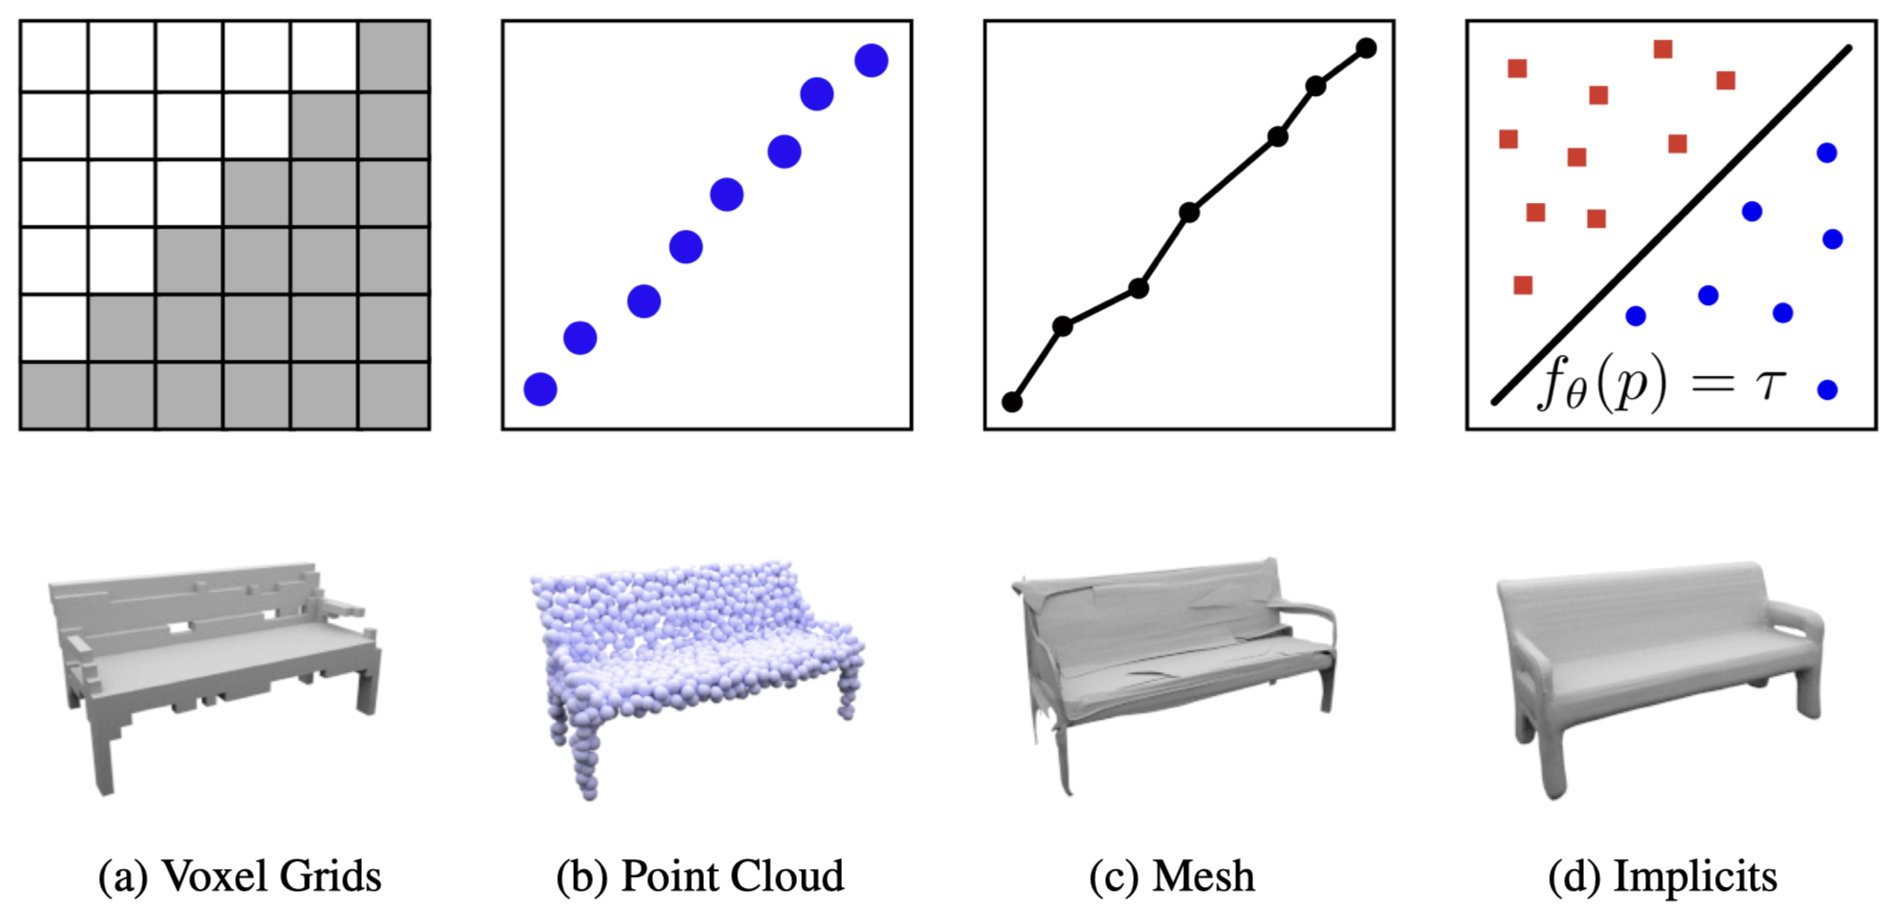
\includegraphics[width=1.0\columnwidth]{imgs/3d_representation.png}
    \caption{Different 3D representations. Image is taken from~\cite{mescheder2019occupancy}.}
    \label{fig:3d_representation}
\end{figure}


\section{Point Cloud Capturing}
\label{sec:bg_pc_caputure}
3D data can be represented in various forms (\cf \cref{fig:3d_representation}), including multi-view images~\cite{su2015multi,qi2016volumetric}, voxels~\cite{wu20153d,maturana2015voxnet}, point clouds~\cite{qi2017pointnet,wang2019dynamic}, polygon meshes~\cite{hanocka2019meshcnn,NEURIPS2020_0a656cc1}, and implicit representations~\cite{mescheder2019occupancy,park2019deepsdf,chen2019learning,yang2021geometry}. Among these, point clouds are favored for their scalability and reduced complexity compared to voxels and meshes, and their explicitness compared to multi-view images and implicit representations. In its simplest form, a point cloud represents 3D geometry as a set of unordered points, where each point encodes the 3D coordinates. Depending on the capturing device, these points may also include color information and intensity values, which provide radiometric information that can be used to infer surface material properties. Various sensors can capture point cloud data, each offering distinct working principles, levels of accuracy, and application scenarios.

\noindent
\textbf{LiDAR (Light Detection and Ranging)} uses laser pulses to measure distances with centimeter-level accuracy. Unlike cameras, LiDAR is an active sensor, meaning it operates independently of ambient light, making it highly reliable for 24/7 operations. With a wide field of view, LiDAR sensors can capture a comprehensive view of the surroundings in all directions simultaneously. These advantages, along with its proven reliability, have made LiDAR a key technology in autonomous driving (AV) and robot navigation. Datasets like KITTI~\cite{geiger2012we}, Waymo~\cite{sun2020scalability}, and nuScenes~\cite{caesar2020nuscenes} are all captured using LiDAR sensors. KITTI and Waymo employ 64-beam LiDAR, while nuScenes uses a 32-beam LiDAR, which offers lower vertical resolution but higher capture frequency (10 Hz for 64-beam versus 20 Hz for 32-beam LiDAR). The resulting LiDAR data typically exhibit a layered pattern, with each layer corresponding to a specific vertical angle. The point cloud is denser near the sensor and becomes sparser at greater distances, which poses challenges for point cloud processing techniques.

\noindent
\textbf{Terrestrial Laser Scanning (TLS)}, similar to LiDAR, operates by emitting laser pulses to measure distances but remains stationary during data collection. This stationary operation results in highly detailed and precise point clouds with millimeter-level accuracy, making TLS ideal for applications requiring fine-grained detail, such as surface reconstruction, building information modeling (BIM), heritage preservation, and structural analysis. Well-known examples of TLS datasets include the Stanford 3D Scanning Repository~\cite{curless1996volumetric} and the ETH ASL point cloud registration dataset~\cite{Pomerleau_2012}.

\noindent
\textbf{RGB-D cameras}, such as Microsoft Kinect and Intel RealSense, integrate standard RGB imaging with depth sensing to capture both color and depth information simultaneously. These cameras typically use either structured light or Time-of-Flight (ToF) technology to generate depth maps, which are then combined with RGB data to create a sparse 3D point cloud with color information. To obtain a dense point cloud, multiple RGB-D frames can be fused using TSDF fusion~\cite{curless1996volumetric,zeng20163dmatch}. While RGB-D cameras are valued for their ability to capture rich 3D data in real-time at relatively low cost and moderate accuracy, typically within a few millimeters, they often face challenges with transparent or highly reflective surfaces. This issue arises because the light used to measure depth can either pass through transparent materials or be reflected away from the sensor, resulting in inaccuracies or gaps in the depth data. Despite these challenges, RGB-D cameras are widely used in robotics, augmented reality, and human-computer interaction. Notable datasets captured using RGB-D cameras include the NYU Depth Dataset~\cite{Silberman_ECCV12}, ScanNet~\cite{dai2017scannet}, and 3DMatch~\cite{zeng20163dmatch}.

\noindent
\textbf{Stereo cameras} capture two or more images from slightly different angles, and by comparing these images, they calculate disparity maps to generate a 3D point cloud. The accuracy of depth estimation depends on the baseline distance between cameras, image resolution, and the stereo matching algorithm. They may struggle in low-light conditions or with featureless surfaces, where establishing correspondences between the images becomes difficult. Stereo cameras are widely used in photogrammetry for 3D reconstruction. Notable datasets include the Middlebury Stereo Dataset~\cite{scharstein2002taxonomy} and ETH3D stereo benchmark~\cite{schops2017multi}.

\section{Point Cloud Processing}
\label{sec:bg_pc_process}
Point cloud data is unordered and unstructured, requiring models to be invariant to $N\!$ permutations and robust to \textbf{SE}(3) transformations. Additionally, point clouds often have varied point density and noise, posing challenges for learning-based models. In this section, we introduce various learning-based methods that handle unstructured point cloud data. For a comprehensive review, refer to Guo \etal~\cite{guo2020deep}.

\paragraph{Point-wise MLP}
DeepSets~\cite{zaheer2017deep} and PointNet~\cite{qi2017pointnet} pioneered deep learning for point cloud processing by introducing permutation-invariant operators. PointNet processes each point individually using shared MLPs, followed by global max pooling to aggregate features, capturing global point cloud characteristics while being invariant to permutations. DeepSets~\cite{zaheer2017deep} achieves permutation invariance by summing all representations and applying nonlinear transformations. PointNet++\cite{qi2017pointnet++} extends PointNet by incorporating hierarchical structures to capture local context and progressively enrich global features. These methods are simple and effective for handling unordered point clouds but may struggle with fine-grained local structures due to the pooling approach. Extensions of PointNet++ improve local structure capture through enhanced neighborhood selection and aggregation techniques~\cite{wang2019dynamic}, as well as scalability~\cite{NEURIPS2022_9318763d}. RandLA-Net\cite{hu2020randla} focuses on real-time large-scale point cloud processing with a random sampling strategy and lightweight local feature aggregation, reducing computational load while maintaining performance.

\paragraph{Point convolution}
To improve the efficiency of local feature aggregation, point convolution methods~\cite{li2018pointcnn,wu2019pointconv,thomas2019kpconv} define convolution kernels for point cloud data, with weights for neighboring points related to their spatial distribution relative to the center point. KPConv~\cite{thomas2019kpconv} introduces kernel points and learns weights for these points to perform convolutions directly on point sets. For varied density or complex geometry, deformable kernel points with learnable shifts are proposed. Compared to point-wise MLP-based methods~\cite{qi2017pointnet,qi2017pointnet++}, KPConv excels in detailed local feature extraction for tasks such as 3D semantic segmentation and representation learning~\cite{bai2020d3feat}. However, tuning the receptive field for different point densities and handling noise can be challenging.

\paragraph{Sparse convolution}
Addressing the inherent sparsity of point cloud data, sparse convolution methods~\cite{tang2022torchsparse,hackel2020inference,3DSemanticSegmentationWithSubmanifoldSparseConvNet} focus on non-empty voxels and preserve sparse structures in deep layers, significantly reducing computational load and memory usage. These methods utilize hash tables to efficiently access active voxels, making them highly efficient for large-scale 3D scene understanding. Compared to point convolution methods, the receptive fields of sparse convolution layers are more intuitive and easier to understand. However, voxelization can lead to loss of fine detail and precision, which may be critical for fine-grained recognition tasks.

\paragraph{BEV projection}
Bird's Eye View (BEV) projection transforms point clouds into a top-down 2D grid representation, simplifying the data structure and making it compatible with traditional 2D convolutional neural networks. This technique is widely used in autonomous driving for tasks like object detection~\cite{zhou2018voxelnet,lang2019pointpillars} and semantic segmentation~\cite{aksoy2020salsanet}, leveraging efficient 2D CNN architectures. The main advantage is computational efficiency and ease of integration with existing 2D CNN frameworks. However, the projection can lead to loss of height information and resolution, potentially affecting 3D feature extraction accuracy. Advanced approaches combine BEV with other local feature aggregations. PointPillars~\cite{lang2019pointpillars} applies PointNet~\cite{qi2017pointnet} within each grid to aggregate local context before applying 2D operations.

\paragraph{Relevance to my works} In~\cref{chap:cvpr21}, we adopt both point convolution~\cite{thomas2019kpconv} and sparse convolution~\cite{choy2019Minkowski} to build the feature extraction backbone. In~\cref{chap:eccv22}, we combine point-wise MLP and BEV projection to handle LiDAR scans captured in street scenes. 


\section{Neural Field in Visual Computing}
\label{sec:bg_neural_field}
Neural fields, also known as implicit neural representations or coordinate-based neural networks, have revolutionized the way we represent and reconstruct 3D shapes and scenes. These neural fields are parameterized, either fully or partially, by neural networks that map points in space and time to physical quantities such as gravity, density, and radiance. This continuous representation allows for representing shapes with arbitrary topology and at infinite resolution, offering superior flexibility and representation capacity compared to its explicit counterparts like point clouds, voxels, and meshes, which often lose detail due to discretization or struggle with complex topologies.

The reconstruction of a neural field typically involves coupling it with a differentiable forward model, which projects the reconstructed domain onto the sensor domain, and is supervised using reconstruction loss. In this section, we explore two applications of neural fields relevant to this thesis: 3D shape modelling and novel view synthesis. For a more comprehensive review, please refer to the work by Xie \etal~\cite{xie2022neural}.

\paragraph{3D Shape modelling}
IM-Net~\cite{chen2019learning}, OccupancyNetwork~\cite{mescheder2019occupancy}, and DeepSDF~\cite{park2019deepsdf} pioneered the modeling of 3D shapes using neural fields. These approaches employ a coordinate-based decoder that takes query coordinates as input and uses a shape code as a condition to estimate occupancy (whether a point is inside or outside the shape)~\cite{mescheder2019occupancy, chen2019learning} or signed distance\cite{park2019deepsdf}. The zero level of the shape is subsequently determined based on these estimates, and the polygon mesh can be reconstructed using methods like Marching Cubes~\cite{levoy1990efficient} or FlexiCubes~\cite{shen2023flexible}.

The decoders in these models are often parameterized as fully connected multilayer perceptrons (MLPs), leveraging the smoothness inductive bias. The shape code can be obtained in different ways. DeepSDF~\cite{park2019deepsdf} uses test-time optimization to derive the shape code, which allows for better generalization since it doesn't make assumptions about the input data. However, this approach may potentially overfit to the input data. In contrast, OccupancyNetwork and IM-Net directly regress the shape code from the input data, making them significantly faster at inference time, though they may not fully capture the fine-grained details of the input. Yang \etal~\cite{yang2023reconstructing} proposed a hybrid approach that combines an explicit encoder with an auto-decoder. This method first regresses the shape code and then refines it using test-time optimization, enhancing robustness to input noise and stabilizing the optimization process. Despite these advancements, all these methods rely on a single global shape code as a condition, which limits their capacity to model fine-grained details.

To address this limitation, several works have proposed conditioning on local shape codes~\cite{peng2020convolutional, jiang2020local, genova2020local, chabra2020deep}. This approach allows implicit representations to scale up to large-scale indoor scenes. For example, the ConvOccNet~\cite{peng2020convolutional} uses a volume encoder and decoder. It first voxelizes the point cloud and extracts voxel features using a small PointNet, then aggregates global features using 3D UNet architectures. For a query coordinate, it interpolates local features from the 3D feature volume and uses a shared decoder to output the occupancy value. By conditioning on local features instead of a global shape code, these methods excel at preserving fine-grained details and generalizing to new scenes or shapes.
% 3D data are often captured and represented in the form of point cloud or multi-view images. How to effectively reconstruct the underlying geometry remains a challenging problem, due to sparse surface sampling, noisy points, varying lighting condition, or small overlap among multi-view images. OccupancyNetwork~\cite{} 


\paragraph{Novel view synthesis}
Given a set of posed images capturing a scene, novel view synthesis involves rendering views from new viewpoints of the same scene. This is an important task due to its numerous applications in fields such as AR/VR, movies, visual effects, virtual try-on, and more. At its core, it addresses a fundamental challenge: effectively representing and reconstructing the underlying 3D scene from images, enabling rendering photorealistic and view-consistent images when projected back to the sensor domain. Previous methods employ various representations such as meshes~\cite{buehler2001unstructured,debevec2023modeling}, depth map warping~\cite{chen2023view,shade1998layered}, multi-plane images~\cite{flynn2019deepview,srinivasan2019pushing}, and volumes~\cite{henzler2018single,Lombardi2019,curless1996volumetric}, each offering unique approaches to reconstruct and render novel views. However, these methods often suffer from limited representation capacity due to the discretization of space, or difficulties during shape optimization.

Neural Radiance Fields (NeRF)\cite{mildenhall2020nerf} provides an alternative solution to circumvent these problems. NeRF represents the 3D scene using a neural field parameterized by a Multi-Layer Perceptron (MLP) network that takes 5D input (3D spatial coordinates and 2D view direction) and outputs density and radiance values. To mitigate the spectral bias\cite{tancik2020fourier} of fully connected networks, which tend to only represent low-frequency signals, NeRF lifts spatial coordinates to high-dimensional Fourier features before feeding them to the MLP. The final pixel is rendered using volume rendering~\cite{levoy1990efficient,max1995optical}, which samples equidistant points along a ray, queries their individual density and radiance values, and integrates the transmitted radiance along the ray. This entire model is fully differentiable, with dense sampling of the 3D space resulting in stable scene optimization. 

NeRF~\cite{mildenhall2020nerf} is slow to optimize due to the dense ray sampling and the deep and wide MLP network required to model large-scale and complex scenes. Follow-up works have improved training efficiency by leveraging explicit feature grids~\cite{mueller2022instant,SunSC22,fridovich2022plenoxels,yu2021plenoxels} or factorized feature planes~\cite{chen2022tensorf,kplanes_2023}. For instance, Instant-NGP~\cite{mueller2022instant} optimizes a fixed-size hash lookup table. For each query point, it indexes the multi-resolution hash encoding according to the corresponding grid corners at each resolution, then linearly interpolates the features based on the coordinates within the grid. Features at different resolutions are concatenated to form the final local feature. Given the sufficient representation capacity of the multi-resolution hash encoding, the NeRF decoder can be a shallow MLP, significantly improving query efficiency. Another key component of Instant-NGP is the fast fully-fused MLPs of the tiny-cuda-nn framework~\cite{tiny-cuda-nn}, reducing training time to seconds. However, rendering efficiency at inference time remains limited by the expensive ray sampling. Gaussian Splatting~\cite{kerbl20233d} further enhances rendering efficiency by replacing volume rendering with rasterization.

\paragraph{Relevance to my works} In ~\cref{chap:iccv23} and ~\cref{chap:cvpr24}, we utilize Instant-NGP as the backbone for our neural LiDAR field. In FEGR~\cite{wang2023neural}, we integrate both neural fields and meshes for inverse rendering tasks. For large-scale scene modeling in ImpliCity~\cite{stucker2022implicity}, we employ ConvOccNet~\cite{peng2020convolutional}. Additionally, in LivingScene~\cite{zhu2023living}, we use DeepSDF~\cite{park2019deepsdf} to model shapes.


\section{Problem statements}
\label{sec:bg_problems}